\section{Livello Rete}
    \subsection{Indirizzi IPv4}
        \subsubsection{Classi}
            \problem
            
            Le classi B sono 16K. Si supponga che invece di utilizzare 16 bit per la casse B se ne fossero utilizzati 20. Quante classi B ci sarebbero state?

            \solution
            256K
        
        \subsubsection{Subnetting 1}
            \problem
            La classe C 192.1.1.0 viene assegnata a tre Dipartimenti A (100 host), B (60 host) e C (40 host), ciascuno con la propria LAN.

            Determinare il subnetting ottimale per questa situazione
            
            \solution
            192.1.1.0/25 (128 indirizzi)\\
            192.1.1.128/26  (64 indirizzi)\\
            192.1.1.192/26 (64 indirizzi)
        
        \subsubsection{Subnetting 2}
            \problem
            Ad una organizzazione viene assegnato il blocco di indirizzi IP 130.56.0.0/16.

            L'amministratore vuole creare 1024 sottoreti con una maschera di sottorete fissa. Determinare:
            \begin{enumerate}
                \item La maschera per le sottoreti.
                \item Il numero di host per sottorete.
                \item Indirizzo di rete e di broadcast della prima e dell'ultima subnet.
            \end{enumerate}

            \solution
            Per avere 1024 sottoreti dobbiamo dedicare 10 bit ($2^{10}$ = 1024) per il subnetting; ne rimangono 6 per gli host (16+10+6 = 32).

            Il numero di host per sottorete è $2^6$-2 = 62
            
            Prima sottorete: 130.56.0.0/26 (X.Y.00000000.00 000000)
            
            Con broadcast: 130.56.0.63 (X.Y.00000000.00 111111)
            
            Ultima sottorete: 130.56.255.192/26(X.Y.11111111.11 000000)
        
            Con broadcast: 130.56.255.255 (X.Y.11111111.11 111111)
        
        \subsubsection{Supernetting}
            \problem
            Un router deve annunciare che gli indirizzi da \verb|10.10.0.0| a \verb|10.10.50.255| e da \verb|10.10.64.0.0| a \verb|10.10.127.255| sono raggiungibili attraverso l'interfaccia 1, mentre gli indirizzi da \verb|10.10.60.0| a \verb|10.10.63.255| sono raggiungibili attraverso l'interfaccia 2.

            Aggregare correttamente gli indirizzi utilizzando il minor numero di reti.

            \solution
            \verb|10.10.0.0/17| (da 10.10.0.0 a 10.10.127.255) int 1\\
            \verb|10.10.60.0/22| (da 10.10.60.0 a 10.10.63.255) int 2
    
    \subsection{Instradamento}
        \subsubsection{Miglior instradamento}
            \problem
            \centerline{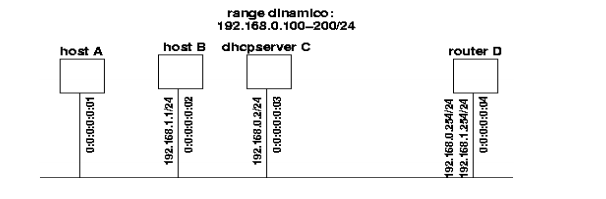
\includegraphics{instradamento}}

            Considerare la configurazione di rete di figura.

            L'host A configurato con indirizzo IP dinamico si accende e invia un ping a B.

            Descrivere la sequenza di tutti i pacchetti che transitano sulla rete dettagliandone il contenuto (indirizzi di mittente e destinatario) a livello 2 e 3.

            Specificare le azioni da intraprendere per migliorare l'instradamento di questi pacchetti.
            
            \solution
            \begin{enumerate}
                \item macA,  0.0.0.0:dhcps $\rightarrow$ bcast:dhcpc  (DHCP discover)

                \item macC, ipC:dhcpc $\rightarrow$ macA, ipA:dhcps (DHCP offer)
                
                \item macA, 0.0.0.0:dhcps $\rightarrow$ bcast:dhcpc (DHCP request)
                
                \item macC, ipC:dhcpc $\rightarrow$ macA, ip A:dhcps (DHCP ack)
                
                \item macA $\rightarrow$ bcast : ARP (query mac HOST D?)
                
                \item macD $\rightarrow$ macA: ARP (reply)
                
                \item macA, ipA $\rightarrow$ macD, ipB: ICMP  (echo-request)
                
                \item macD $\rightarrow$ bcast, ARP (query mac HOST B?)
                
                \item macB $\rightarrow$ macD, ARP (reply)
                
                \item macD, ipA $\rightarrow$ macB, ipB:ICMP (echo-request)
                
                \item macB, ipB $\rightarrow$ macD, ipA:ICMP (echo-reply)
                
                \item macD, ipB $\rightarrow$ macA, ipA:ICMP (echo reply)
            \end{enumerate}

            Il passaggio dal router può essere evitato configurando route statiche su host A e host B.

            host A: 192.168.1.0/24 * (consegna diretta)

            host B: 192.168.0..0/24 * (consegna diretta) 

            In questo modo non vengono generati i pacchetti 8, 9,  10 e 12

            Nel pacchetto 5 la query sarebbe per HOST B  al posto di HOST D.

        \subsubsection{NAT}
            \problem
            \centerline{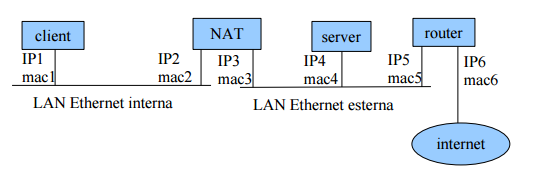
\includegraphics{nat}}
            Si consideri la rete di figura in cui:
            \begin{itemize}
                \item Il client ha un indirizzo privato IP1 e un default router IP2.
                \item Il server ha un indirizzo pubblico IP4 e un default router IP5.
            \end{itemize}

            Subito dopo l'accensione delle macchine il client genera \verb|ping IP4|.

            Elencare tutti i frame conseguenti al ping, dettagliando per ogni frame la stratificazione dei protocolli utilizzati e le relative informazioni principali.

            \solution
            \begin{enumerate}
                \item mac1 $\rightarrow$ bcast LAN interna: ARP (query mac IP2?)

                \item mac2 $\rightarrow$ mac1: ARP reply

                \item mac1, IP1 $\rightarrow$ mac2, IP4: ICMP (echo-request)

                \item mac3 $\rightarrow$ bcast LAN esterna: ARP (request mac IP4 ?)

                \item mac4 $\rightarrow$ mac3: ARP (reply)

                \item mac3, IP3 $\rightarrow$ mac4, IP4:ICMP (echo-request)

                \item mac4, IP4 $\rightarrow$ mac3, IP3:ICMP (echo-reply)

                \item mac2, IP2 $\rightarrow$ mac1, IP1:ICMP (echo-reply) 
            \end{enumerate}

    \subsection{Routing}
        \subsubsection{Routing 1}
            \problem
            \centerline{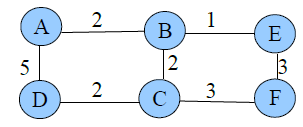
\includegraphics{routing}}

            Per la rete di figura indicate le tabelle di routing a regime con i seguenti dati:
            Destinazione - (costo, NextHop)
            Si supponga che ad un certo istante:
            \begin{itemize}
                \item Il link BE si interrompe.
                \item I nodi B ed E si accorgono del disservizio.
            \end{itemize}

            Descrivere il comportamento del routing per i nodi B ed E nel caso si utilizzi:
            \begin{itemize}
                \item Il protocollo Distance Vector (DV scambiati, nuove tabelle di routing).
                \item Il protocollo Link State (LSP scambiati, nuove tabelle di routing).
            \end{itemize}

        \subsubsection{Routing 2}
            \problem
            \centerline{A ----- B ----- C}
            
            Si consideri una sottorete lineare composta da 3 nodi disposti come in figura, in cui è abilitato un protocollo di Routing dinamico con un costo 1 tra nodi adiacenti.
            \begin{enumerate}
                \item Supponendo di aggiungere un quarto nodo D connesso a C stabilire il numero di
                scambi necessari per aggiornare le tabelle di instradamento e calcolare ad ogni
                scambio la distanza da D per ogni nodo per i protocolli di tipo "Distance Vector" e
                "Link State"
                \item Supponendo di eliminare nuovamente il nodo D, descrivere la dinamica delle
                tabelle nella nuova situazione per entrambi i protocolli e discutere le differenze
            \end{enumerate}